\documentclass[12pt, titlepage]{article}

\usepackage[margin=1in]{geometry}
\usepackage[
    citestyle=authortitle,
    autocite=footnote
]{biblatex}
    \addbibresource{bibliography.bib}
\usepackage{float}
\usepackage{amsfonts}
\usepackage{amssymb}
\usepackage{amsmath}
\usepackage{amsthm}
    \newtheorem{theorem}{Theorem}
    \newtheorem*{definition}{Definition}
\usepackage{array}
\usepackage{graphicx}
    \graphicspath{{media/}} 
\usepackage[
    colorlinks,
    linkcolor=black,
    citecolor=black,
    urlcolor=blue
]{hyperref}
\usepackage{enumitem}
\usepackage{tikz}
    \usetikzlibrary{positioning}
\usepackage{fontenc}
\usepackage{setspace}

\setlength{\parskip}{1em}
\setlength{\parindent}{0em}

\font\titlefont=cmr12 at 36pt

\let\oldsection\section
\renewcommand\section{\clearpage\oldsection}

\begin{document}

\begin{titlepage}
    \topskip0pt
    \vspace*{\fill}
	\centering

    {\titlefont HOW DOES THE}\\[0.5cm]
    {\titlefont INTERNET STAY}\\[0.5cm]
    {\titlefont SECURE?}

    \vspace{2.5cm}
    
\includegraphics[scale=0.8]{title_image}
    \vspace{2.5cm}

    {\Large Mathematics HL} \\
    \vspace{0.5cm}
    {\Large gcw615}\\
    \vspace{0.5cm}
    {\Large Examination Session: May 2017} \\
    \vspace{0.5cm}
    {\Large Word Count: }
    \vspace*{\fill}
\end{titlepage}

\section*{Abstract}

Public key encryption schemes are essential to ensuring the security of the modern internet.
This extended essay explores one of the most used such schemes, RSA, through the research
question of how \textbf{RSA allows for secure and private communication over the internet}.
Initially, the basic idea behind public key encryption is explained. Prime numbers and
modular arithmetic, two concepts necessary for understanding the main proofs, are
introduced. A number of primality tests which can be used for generating prime numbers for
use in RSA encryption, namely, trial division, the Sieve of Eratosthenes and the Fermat Test
are explained. The mathematics behind RSA encryption, namely Euler's Theorem, will be
addressed, and a proof of RSA's correctness will be provided through showing that any given
message can be encrypted and then decrypted and remain intact. The research question is
finally answered by showing that it is extremely difficult --- practically impossible with
current technology --- to find the private key of an RSA key pair knowing only the public
key.  Furthermore, the possibility of using Mersenne prime numbers as the base primes for
RSA encryption will be discussed, an idea which is quickly disregarded due to the triviality
of exhaustively testing every single pair of Mersenne primes, as only 49 such primes have
been discovered.  

Word count: 211

\thispagestyle{empty}

% No page number for ToC
\addtocontents{toc}{\protect\thispagestyle{empty}}
% Add intro to ToC even if it has no page number
\addcontentsline{toc}{section}{\nameref{sec:intro}}
\tableofcontents

\section*{Introduction}

% Start numbering from Introduction page
\setcounter{page}{1}
\label{sec:intro}

People have always wanted to exchange secret messages. From ancient times, methods such as
the Caesar cipher --- which substitutes each letter in a message with the one a number of
letters forward in the alphabet --- have been used to achieve that goal, and were the first
steps in the study of cryptography. These methods have all had a shared characteristic: they
needed their users to share a secret key.

In modern cryptography, however, it is often necessary to exchange messages without having
the chance of exchanging such a key; think encrypting a password entered into a website you
are visiting for the first time. It is out of this necessity that the idea of public key
cryptography was born. What this allowed was for two parties to exchange messages securely
without ever having to exchange any secret information. Even if a third party were to listen
in on all communications between them, they would still be unable to understand the messages
they were exchanging.

The main idea behind public key cryptography is that encryption (changing a message into an
unreadable form) and decryption (the inverse operation of encryption, recovering the
original message from the unreadable form) don't have to use the exact same key: there can
be a pair of keys, one used for encryption and the other for decryption. Say Alice wants to
send a message to Bob and they each have an encryption key and a decryption key. Bob can
publicly share his encryption key which Alice will then use to encrypt the message she wants
to send, and send the encrypted message to Bob. When he receives it, he can use his
decryption key to decrypt the message. Because of the way they are used, the encryption key
is often called the \emph{public key} and the decryption key the \emph{private key}
%
\begin{figure}[h!] 
    \centering
    \label{fig:message_exchange}
    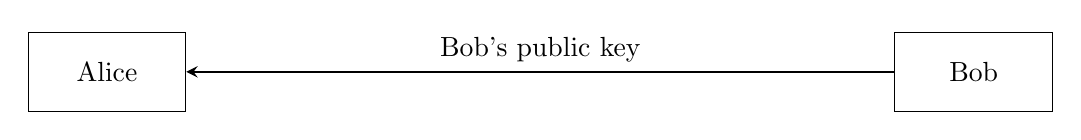
\begin{tikzpicture}[>=stealth]
        \tikzstyle{character}=[rectangle, draw, minimum height=1cm, minimum width=2cm];

        \node (A) [character] {Alice};
        \node (B) [character, right=10cm] {Bob};
        \draw[->, thick] (B) -- node[above]{Bob's public key} (A);
    \end{tikzpicture}
    
    \vspace{1cm}
    Alice encrypts message using Bob's public key
    \vspace{1cm}

    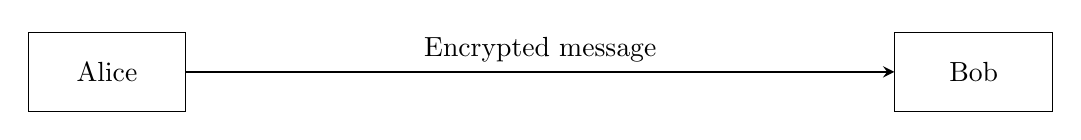
\begin{tikzpicture}[>=stealth]
        \tikzstyle{character}=[rectangle, draw, minimum height=1cm, minimum width=2cm];

        \node (A) [character] {Alice};
        \node (B) [character, right=10cm] {Bob};
        \draw[->, thick] (A) -- node[above]{Encrypted message} (B);
    \end{tikzpicture}

    \vspace{1cm}
    Bob decrypts message using his private key
    \vspace{1cm}

    \caption{Exchanging an encrypted message using public key cryptography}
\end{figure}
%

Even if someone were to intercept both communications, they would still have no access to
the original message

I have been interested in computers and programming from a very young age, and so I have
recently made a few websites as personal projects. Since these websites required the users
to create an account and provide a password, it was necessary that the communication between
the user's computer and the server was encrypted. This, however, was handled automatically
from the server using a public key encryption scheme called \emph{RSA}. All I had to do was
generate a key pair and configure the server to use that key pair whenever the website was
accessed.  Therefore, all the underlying mathematics of RSA encryption were hidden. Since
this encryption scheme was such an important part of my personal projects as well as the
entire internet, I became interested in how it works beneath the surface and how it can be
rigorously proven that a scheme like this is "secure". This led to my research question:
\textbf{How does RSA allow for secure and private communication over the internet?}

In my essay I will focus on the mathematics behind RSA (consisting mainly of number theory),
aiming to explore its proof of correctness. In the first section of my essay, I will
introduce prime numbers, central to the area of number theory and to RSA specifically, as
well as the concepts of linear congruences, which is what the proof of RSA is based on, and
of residue systems and classes, which will help simplify some of the other proofs provided
in the essay. In the second section, I will introduce a number of so-called primality tests,
which are used in the generation of keys for RSA, including trial division, the Sieve of
Eratosthenes, and the Fermat test. In the third and final part of the essay I will answer my
research question by providing a proof of correctness for RSA, and showing that it does,
indeed, ensure that communication using it is secure.

\section{Divisibility}

\subsection{Prime numbers}

Prime numbers are one of the most fundamental concepts in number theory. A prime number is
defined as an integer that can only be exactly divided by $1$ and itself.

An interesting property of prime numbers is that there is an infinite number of them. 
%
\begin{theorem}[Euclid's Theorem]
    The set of all prime numbers is infinite.
\end{theorem}
%
This was was shown by Euclid in his work \emph{Elements}, in a particularly elegant
proof\autocite[19]{dence}:

Suppose the number of primes is finite. Let us label them $p_1, p_2, \ldots, p_n$. Then,
consider the numbers $P = p_1\times p_2\times \ldots \times p_n$ and $q = P + 1$. There are
now two possible cases regarding $P$ and $q$:
%
\begin{enumerate}[label=\alph*)]
    \item $q$ is prime and therefore there is a prime ($q$) that is not contained in the
        initial list, which supposedly contained all primes, or
    \item $q$ is not prime and there exists some prime $p$ which divides $q$. If $p$
        were in the list then it would also divide $P$. But that would mean that it
        would also divide the difference of $P$ and $q$, which is $P - q = P - (P + 1) =
        1$. But no prime divides $1$.  Therefore, $p$ does not divide $P$ and so is not
        in the original list.
\end{enumerate}
%
In both cases, there exists a prime number which is not contained in the original list.
This means that it is not possible to create a (finite) list of all prime numbers since any
such list will be incomplete.
    
A concept related to prime numbers that also often comes up in number theory and RSA in
particular, is that of \emph{relatively prime} or \emph{coprime} numbers. This refers to
numbers which do not share any divisors other than 1.

\textit{Two integers $a, b$ are relatively prime (coprime) if and only if their greatest common
divisor is equal to 1 ($\gcd(a, b) = 1$)}

So, for example, 8 and 15 are coprime, since 8 can be only by divided by 1, 2, 4, and 8,
while 15 can only be divided by 3 and 5. 15 and 9 are not, since 3 divides both.

\subsection{Modular Arithmetic}

An understanding of linear congruences and modular arithmetic is necessary for the
main proofs of the essay.

Linear congruences have to do with division remainders. 

\textit{When two integers $a, b$ are congruent modulo a third integer $m$ they leave the same
remainder when divided by $m$ \autocite[278]{haese_ib_options}. Formally:}
%
\begin{equation}\label{eq:congr_def_long}
    \begin{gathered}
        a \equiv b \pmod{m} \iff \\
        \exists\ l,m,r \in \mathbb{Z}: a = qm + r\ and\ b = lm + r
    \end{gathered}
\end{equation}
%
So, for example, $4 \equiv 7 \pmod{3}$ since both 4 and 7 leave the same remainder, equal to
1, when divided by 3.

An alternate definition is that
%
\begin{equation*}
    a \equiv b \pmod{m} \iff m | a-b
\end{equation*}
%
These two definitions are equivalent. This can be shown starting
from~\eqref{eq:congr_def_long}
%
\begin{equation*}
    \left. 
        \begin{aligned}
            a = qm + r\\ 
            b = lm + r
        \end{aligned}
    \right\}
    \text{Therefore, } (a - b) = (q-l)\times m :\: (q-l) \in \mathbb{Z}\quad
\end{equation*}
%
Which is equivalent to $m | (a-b)$.

\textit{If two integers a,b satisfy $a \equiv b \pmod{m}$, then we say that $b$ is the residue of
$a$ modulo m. Generalising this to all integers, we can state, that all integers are
congruent to one of the possible values of $b$, namely, one of the set $\{0, 1, 2, 3, \ldots,
(n-1)\}$. This set is called \textbf{the complete system of residues modulo
$\mathbf{m}$}}. \autocite[85]{dence}

When performing arithmetic inside a modulo, addition, subtraction, and multiplication behave
exactly as one would expect. Namely, given
$a\equiv b\pmod{m}$ and $c\equiv d\pmod{m}$:
%
\begin{align*}
    a + c &\equiv b + d \pmod{m}\\
    a - c &\equiv b - d \pmod{m}\\
    ka 	  &\equiv kb \pmod{m},\ \text{for all } k \in \mathbb{Z}
\end{align*}
%
Division, however, must be treated using different rules. These will be referred to as the
\emph{Cancellation Laws}\autocite[280]{haese_ib_options}:
%
\begin{gather*}
    \text{Given } d = \gcd(k, m)\\
    kx \equiv ky \pmod{m} \implies x \equiv y \pmod{\frac{m}{d}}
\end{gather*}
%
Note, that if $\gcd(k, m) = 1$, i.e. if we are dividing by a number relatively prime to the
modulo, this simplifies to:
%
\begin{equation*}
    kx \equiv ky \pmod{m} \implies x \equiv y \pmod{m}
\end{equation*}
%

\section{Primality tests}

RSA is based on using very large random primes as the basis of its encryption keys. It is
therefore necessary to have a method of finding such large primes. There is no known way of
directly generating random primes, and so the best way of doing so is generating
progressively larger numbers and checking whether they are prime. In order to achieve that,
a number of so called \emph{primality tests} have been devised  

\subsection{Trial division}

This is perhaps the most intuitive of all the primality tests. It consists of simply of
checking whether a number $p$ (the one being tested as prime) is divisible by all primes
between 1 and $p$. This test however is grossly inefficient, due to the number of trial
divisions that have to be performed for larger integers. There exists however one crucial
theorem that provides an optimisation to this test \autocite[276]{haese_ib_options}:
%
\begin{theorem} \label{th:prime_factors_less_than_root}
    All composites have a prime factor less than or equal to their square
    root. Formally:\\
    $$\forall \text{ composite } n \: \exists \text{ prime } p:p|n \: \& \: p \leq \sqrt{n}$$
\end{theorem}
%
%
This means that is enough to check all primes less than $\sqrt{n}$ for whether they divide
$n$, to ensure that $n$ is prime. 

But why is that? Let us examine a composite number $n$

Since $n$ is composite, $n=ab$ for some integers $a, b$ such that $1<a<n$ and $1<b<n$.\\
Suppose $a>\sqrt{n}$ and $b>\sqrt{n}$. Then, $ab>n$ which implies that $n>n$. \\
This is obviously false and so the assumption that both $a,b > \sqrt{n}$ is false as well.

Therefore, $a \leq \sqrt{n}$ or $b \leq \sqrt{n}$. \\
Suppose (without loss of generality) that $a \leq \sqrt{n}$.\\
There exists prime $p: p|a$. (Note, that if $a$ is prime, $p = a$, but this does not
affect the proof.)\\
$p|a$ and $a|n \implies p|n$. But $p|a$, Therefore,  $p \leq a \leq \sqrt{n}$\\

For example, to find the prime factors of 96, you would only have to test the primes between
2 and $\sqrt{96} \approx 9.8$, so the primes between 2 and 9. Trying each of these numbers
gives the following:
%
\begin{align*}
    \frac{96}{2} &= 48 &\frac{96}{5} &= 19.2 \\
    \frac{96}{3} &= 32 &\frac{96}{7} &\approx 13.7\\
\end{align*}
%
So, the prime factors of 96 are 2 and 3.

Even with this optimization, trial division is still slow for very large numbers 

\subsection{Sieve of Eratosthenes}

This method allows for very quick computation of all primes up to a certain limit. Here is
how it works \autocite{wikipedia_eratosthenes_animation}:
%
\begin{enumerate}
    \item Write down all numbers up to the limit you have set.

        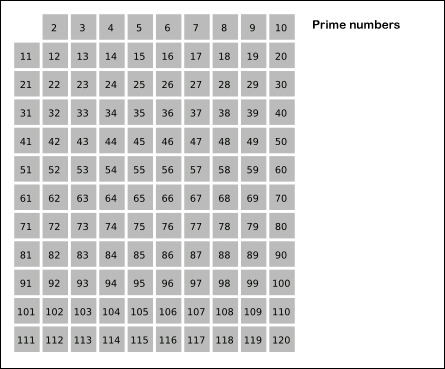
\includegraphics[scale=0.6]{base}
    \item Starting with 2, mark all its multiples, and note 2 as a prime

        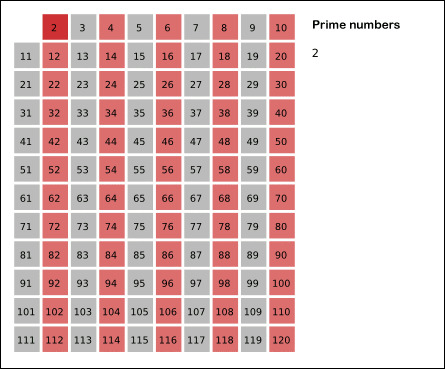
\includegraphics[scale=0.6]{2}\\
    \item Repeat the same process, skipping any marked numbers, and marking
        as prime each unmarked number you encounter

        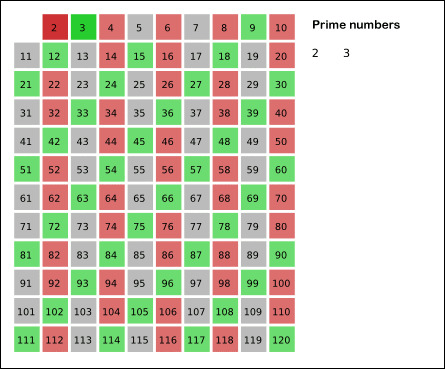
\includegraphics[scale=0.6]{3}\\
        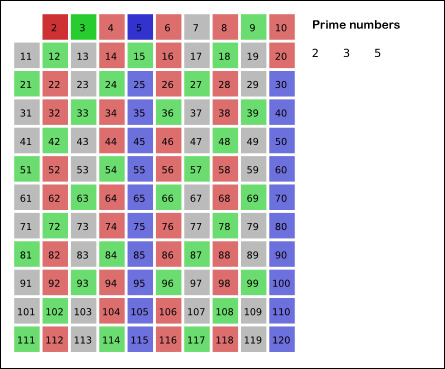
\includegraphics[scale=0.6]{5}\\
        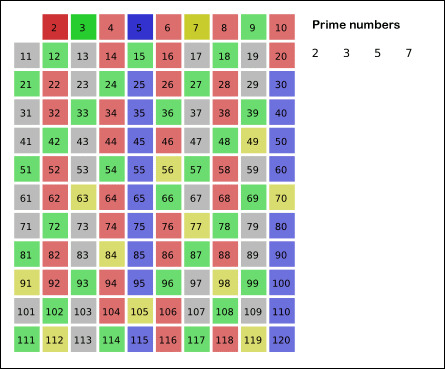
\includegraphics[scale=0.6]{7}\\
\end{enumerate}
%
This method is extremely effective in finding prime numbers, and can even be performed
by hand for moderately small numbers. However, when applied to very large large limits,
the method quickly presents a problem of the memory required. In order for the sieve to
work all found composites must be stored, so that they can be skipped. The memory space
required for the algorithm increases with the limit set, making it impractical for
computing very large primes.
       
\subsection{Fermat test} \label{sec:fermat}

\subsubsection{Fermat's Little Theorem}

Fermat's theorem (not to be confused with Fermat's \emph{last} theorem, its better known big
brother) states that:
%
\begin{theorem}[Fermat's Little Theorem]
    $p$ is prime and $p \not|\ a$ $\implies a^{p-1} \equiv 1 \pmod{p}$
\end{theorem}
%
\begin{proof}
    Consider the numbers 0, 1a, 2a, ..., (p-1)a\\
    Suppose two of them $ka,\ la: 1\leq k < l \leq (p-1)$ are congruent modulo $p$, i.e.
%
    \begin{align*}
              ka &\equiv la \pmod{p}\\
        \iff  k  &\equiv l  \pmod{p} &&\text{since $p$ prime and $p \not| a$}
    \end{align*}
%
    But the integers in $[0, (p-1)]$ form a complete residue system modulo $p$, and  $1
    \leq k<l \leq (p-1)$, meaning that $k \not\equiv l \pmod p$. \emph{Contradiction}.
    Therefore,
%
    \begin{equation*}
        ka \not\equiv la \pmod{p}\qquad \forall\ k,l \in [0, (p-1)], k \not= k
    \end{equation*}
    %
    So, $0...(p-1)a$ are all incongruent to each other and so must be, in some order,
    congruent to the least residue system modulo $p$, i.e.  $0...(p-1)$
%
    \begin{align*}
        a(2a)...(p-1)a &\equiv 1\times 2\times 3...\times (p-1) \pmod{p}\\
        a^{p-1}(p-1)!  &\equiv (p-1)!                           \pmod{p}\\
        a^{p-1}        &\equiv 1                                \pmod{p}
    \end{align*}
\end{proof}
%
(Theorem and proof from \cite[109]{dence})

\subsubsection{Fermat Test}

Based on Fermat's theorem, a primality test can be devised.

Given an even integer $n$ that we want to test for primality we can check whether $a^{n-1}
\equiv 1 \pmod{n}$ holds for a number of integers $1<a<n$.  This test cannot, by itself,
prove the primality of a given number. It can, however, prove compositeness: if $a^{n-1}
\not\equiv 1 \pmod{n}$ then $n$ is necessarily composite since Fermat's theorem holds for
all primes. \cite{primality_akalin}

For example, let us test the number 13 for with the Fermat test, using the bases 5 and 8
(chosen randomly):
%
\begin{align*}
    5^{13-1} = 244140625   \equiv 1 \pmod{13}\\
    8^{13-1} = 68719476736 \equiv 1 \pmod{13}
\end{align*}
%
So, 13 appears to be prime. Further testing with all the bases between 1 and 13 will confirm
that 13 is definitely prime.

Let's also test the Fermat test on a composite number, such as 15, using the base 6
%
\begin{align*}
    6^{15-1} = 470184984576 \equiv 6 \pmod{15}
\end{align*}
%
There is, however, a set of integers called the \emph{Carmichael numbers}, which pass the
Fermat test with any possible base, even though they are composite. Carmichael numbers are,
indeed, rare, they are however infinite. \autocite[116]{dence}

\subsection{The Euler totient function}

This function is necessary for Euler's theorem and, subsequently, RSA encryption. The
definition of the function is quite simple.
%
\begin{definition}
    $\phi(\mathbf{n})$ is defined as the \emph{number} of integers $\mathbf{m}$ less than or
    equal to $\mathbf{n}$ for which $\gcd(m, n) = 1$
\end{definition}
%
So, for example, $\phi(10)$ is 4 since 
%
\begin{align*}
    \gcd(1, 10) &= \mathbf{1} &\gcd(6, 10) &= 2\\
    \gcd(2, 10) &= 2          &\gcd(7, 10) &= \mathbf{1}\\
    \gcd(3, 10) &= \mathbf{1} &\gcd(8, 10) &= 2\\
    \gcd(4, 10) &= 2          &\gcd(9, 10) &= \mathbf{1}\\
    \gcd(5, 10) &= 5          &\gcd(10, 10) &= 10
\end{align*}
%
A quick conclusion that can be drawn is the following:

\textit{For prime $p$, $\phi(p) = p - 1$, since all integers less than or equal to $p$,
aside $p$ itself, are relatively prime to $p$.} 

A plot of the function in \autoref{fig:phi_graph} shows this clearly:
%
\begin{figure}[H]
    \centering
    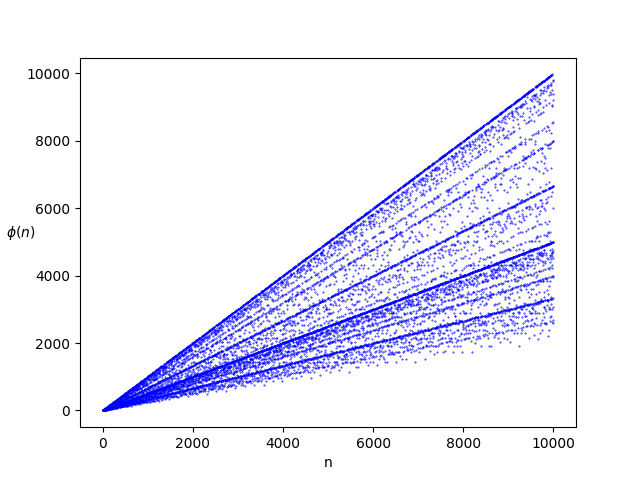
\includegraphics[width=\textwidth]{phi_10000}
    \caption{Graph of $\phi(n)$ for $n$ up to 10000}
    \label{fig:phi_graph}
\end{figure}
%
There is a clear upper bound on the function which follows the line $\phi(n) = n-1$

\subsection{Euler's Theorem}

\begin{theorem}[Fermat's Little Theorem]
    If $m>1$ and $\gcd(a, m) = 1$, then $a^{\phi(m)} \equiv 1 \pmod m$
\end{theorem}

\section{RSA encryption}

RSA \autocite{rsa} is currently, one of the most popular encryption systems in the world.
It belongs to a category of encryption systems known as public-private key.  This means,
that it allows two users to exchange information securely, without having to exchange a
shared encryption key beforehand, as it would be required by classical encryption systems
such as Caesar or substitution ciphers. 

The system is based on the theory of congruences, and, specifically, on Euler's Theorem.

\subsection{Definitions \& Terminology}

Given here are some terms and definitions that will be used:
%
\begin{table}[H]
    \begin{tabular}{ | m{5em} | p{30em} | }
        \hline
        Term      & Definition\\
        \hline
        plaintext & The message that will be encrypted, in \emph{plain
                    text}, i.e. before it is encrypted. Usually represented as $M$\\
        \hline
        ciphertext & The message after it has been encrypted. This is what
                     is sent from one user to the other. Without
                     knowledge of the public and private key it is
                     impossible to recover the plaintext using just the
                     ciphertext. Usually represented as $C$\\
        \hline
    \end{tabular}
\end{table}
%

\subsection{Encryption \& Decryption}

\subsubsection{Keys}

RSA requires a number of values that will be used for the encryption/decryption, known as
keys.  The first of these are two primes \pmb{$p$},\pmb{$q$}. These are usually very large
numbers, in the order of a few hundred or even thousand digits, but for these examples we
will use much smaller primes, just for the sake of simplicity. Next we assign $\pmb{n}=p
\times q$.  Finally, we need an integer \pmb{$e$} such that $gcd(e, \phi (n)) = 1$ and its
multiplicative inverse modulo $\phi(n)$, i.e. an integer \pmb{$d$}, such that $ed \equiv 1
\pmod{\phi(n)}$

The pair $(e, n)$ forms the public or encryption key and the pair $(d, n)$ the private or
decryption key.

\subsubsection{Example}

The values we will use for the example are: $p=13$, $q=11$, $n=143 \implies \phi (n) =
120$, $e = 23$ and $d = 47$

Let's begin with the encryption of a plaintext message. Firstly, the message must be encoded
as a number. The simplest way of doing that would be by converting character into a number
in the residue class modulo $n$ ---i.e. an integer between $0$ and $n-1$, inclusive--- and
encrypting each character separately.  In real world applications, due to the complicated
nature of the arbitrary messages that have to be transmitted, this encoding cannot be used,
but it will suffice for this example.

So, for example, the message "HELLO" would become $8\ 5\ 12\ 12\ 15$, using two digits for
each character.

Next, comes the actual encryption. With $C$ as the ciphertext and $M$ as the plaintext:
\begin{equation*}
    C \equiv M^{e} \pmod{n}
\end{equation*}

Using the keys we defined, the ciphertext becomes $83\ 125\ 12\ 12\ 20$, which can then be
safely transmitted, so that it can be decrypted.   

When the ciphertext is received, the message can be recovered using the congruence
\begin{equation*}
    M \equiv C^{d} \pmod{n}
\end{equation*}

Applying this to the ciphertext of our example, we get $8\ 5\ 12\ 12\ 15$, i.e. our original
message

\subsubsection{Proof}

In order to demonstrate the validity of the encryption scheme it would be worth providing a
formal proof. \autocite{so_rsa_proof}

In order to show that we have to demonstrate that encrypting and decrypting a message gives
back the original value. With $C$ as the ciphertext and $M$ as the plaintext, as well as $C
\equiv M^e \pmod{n}$ for the encryption and $M \equiv C^d \pmod{n}$, what we have to show is
that
%
\begin{align*}
    C^d     &\equiv M \pmod{n}\ \iff \\
    (M^e)^d &\equiv M \pmod{n}\ \iff \\
    M^{ed}  &\equiv M \pmod{n}
\end{align*}
%
From how we have defined our keys we also have the following assumptions:
%
\begin{enumerate}
    \item $p,q\ \text{prime}$
    \item $n = p \cdot q$
    \item $\gcd(e, \phi(n)) = 1$ 
    \item $ed \equiv 1 \pmod{n}$
\end{enumerate}
%
There are two possible cases regarding $M$:
%
\begin{enumerate}
    \item $\gcd(M, n) = 1$
    \item $\gcd(M, n) \not= 1$
\end{enumerate}
%
In the first case, $M^{\phi(n)} \equiv 1 \pmod{n}$ by Euler's theorem. Also the assumption
$ed \equiv 1 \pmod{\phi(n)}$ can be restated as $ed = 1 + k\phi(n)$, for some $k \in
\mathbb{Z}$. So, 
%
\begin{align*}
    M^{ed} &\equiv M^{1 + k\phi(n)} \pmod{n} \\
           &\equiv M \cdot (M^{\phi(n)})^k  \pmod{n} \\
           &\equiv M \cdot 1^k \pmod{n} \\
           &\equiv M \pmod{n}
\end{align*}
%
So the encryption scheme works in the first case

In the second case, there are only two sub cases, since $n = p \cdot q$ where $p, q$ are
both prime, and $ M \in \left[0, n-1\right]$
%
\renewcommand{\labelenumi}{2\alph{enumi}.}
\begin{enumerate}
    \item $\gcd(M, n) = p$
    \item $\gcd(M, n) = q$
\end{enumerate}
%
By the Chinese Remainder Theorem,
%
\begin{equation*}
    \left.
        \begin{aligned}
            M^{ed} &\equiv M \pmod{p}\\
            M^{ed} &\equiv M \pmod{q}
        \end{aligned}
    \right\}
    M^{ed} \equiv M \pmod{pq} \iff M^{ed} \equiv M \pmod{n}
\end{equation*}
%
So, we simply have to show that $M^{ed} \equiv M \pmod{q}$ --- since $p$ and $q$ are
interchangeable --- to prove that $M^{ed} \equiv M \pmod{n}$. This also means that the two
sub cases (2a, 2b) are equivalent. We will be using the sub case $gcd(M, n) = p$ for the
proof.

Since $\gcd(M, n) = p$; $\gcd(M, q) = 1$, and so, by Euler's Theorem,
%
\begin{equation} \label{eq:M-q-euler} 
    M^{\phi(q)} \equiv 1 \pmod{q} 
\end{equation}
%
Also, since, by assumption $ed \equiv 1 \pmod{\phi(n)}$
%
\begin{align*}
    ed - 1 &= h\phi(n) &&\text{for some } h \in \mathbb{Z}\\
    ed - 1 &= h(p-1)(q-1)
\end{align*}
%
Going back to the statement that we have to prove (i.e. $M^{ed} \equiv M \pmod{q}$):
%
\begin{align*}
    M^{ed} &\equiv M^{ed - 1} M \pmod{q} \\
           &\equiv M^{h(p-1)(q-1)} M \pmod{q} \\
           &\equiv (M^{(q-1)})^{h(p-1)} M \pmod{q} \\
           &\equiv (M^{\phi(q)})^{h(p-1)} M \pmod{q} &&\text{Since $q$ is prime,
           meaning that $\phi(q) = q-1$} \\
           &\equiv 1^{h(p-1)} M \pmod{q} &&\text{From (\ref{eq:M-q-euler})}\\
           &\equiv M \pmod{q}
\end{align*}
%
As stated before, this is enough to prove the validity of the second case, and so of RSA as
a whole.

\subsection{Key generation}

It is also worth looking into how the keys necessary for the encryption, as it is not a
trivial process.

The first necessary step is generating the two primes \pmb{$p$} and \pmb{$q$} that form the
basis of the key. There are a number of processes for generating (pseudo-)random numbers
which are outside the scope of this essay. In order to generate a random prime number, one
would use such a technique to generate an odd random number and test it for primality.  If
it is not prime increment by two and repeat until a prime number is found:
%
\begin{figure}[H]
    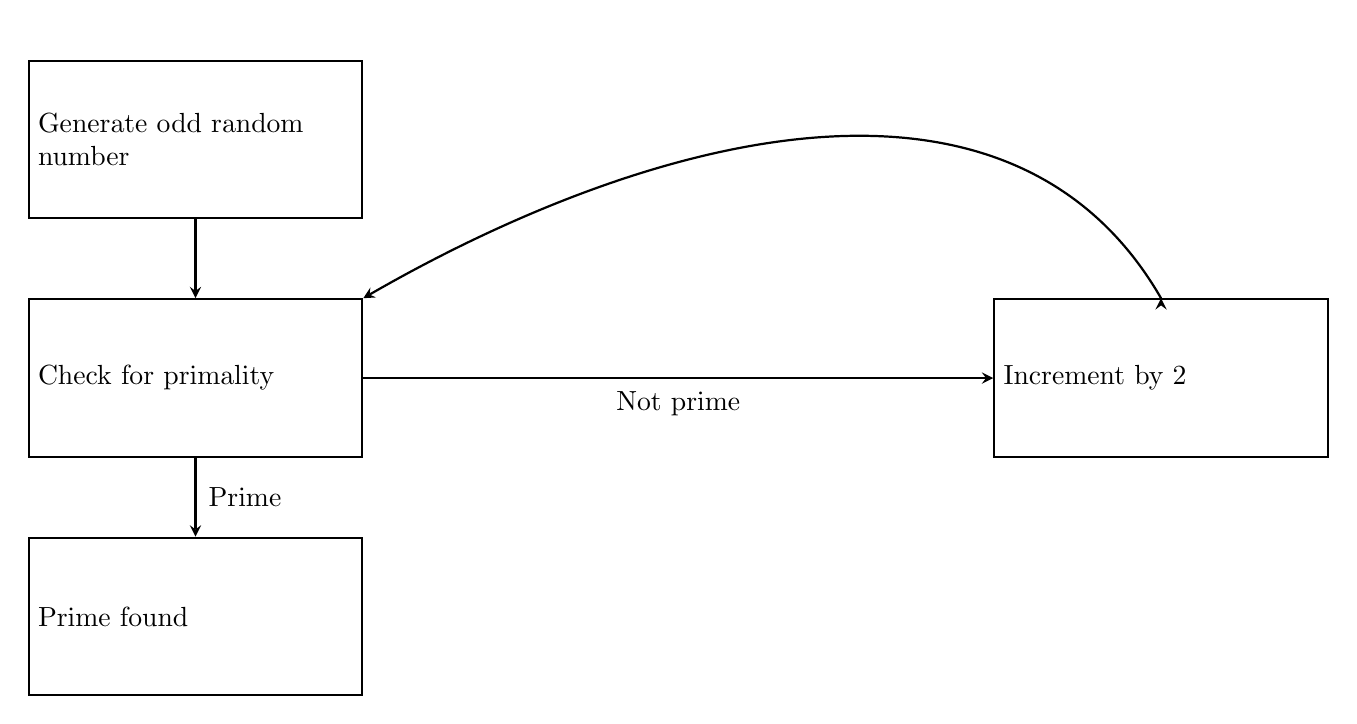
\begin{tikzpicture}[->, >=stealth, thick, main node/.style={rectangle, draw,
        minimum height=2cm, text width=4cm}]
        \node[main node] (generate) {Generate odd random number};
        \node[main node, below = of generate] (check) {Check for primality};
        \node[main node, right = 8cm of check] (increment) {Increment by 2};
        \node[main node, below = of check] (end) {Prime found};

        \draw (generate) -- (check);
        \draw (check.south) -- (end) node[midway, right=1pt] {Prime};
        \draw (check.east) -- (increment.west) node[midway, below=1pt] {Not prime};
        \draw (increment.north) edge[out=120, in=30] (check.north east);
    \end{tikzpicture}
\end{figure}
%
At the core of this process lies the \emph{primality test}. Since they keys used for RSA are
often 512 or even 1024 bit numbers (meaning they can take values of up to $2^{512} - 1$ or
$2^{1024} - 1$ respectively) using trivial primality tests such as trial division or even
the Sieve of Eratosthenes would take far longer than would be deemed practical.  For this
reason, so-called probabilistic primality tests are used. These tests are much faster but
sometimes provide false positives, meaning that they will classify composite numbers as
prime. Examples of such tests include the Fermat, AKS, and Miller-Rabin tests. The simplest
of these is the Fermat test --- which has been explained in \autoref{sec:fermat} --- 

Then \pmb{$n$} is computed as the product of $p$ and $q$. $$n=p \cdot q$$

Finally, \pmb{$k$} is chosen to be an odd random integer, relatively prime to $\phi(n)$,
since $n=p \cdot q$ and $p,q$ prime, $\phi(n) = \phi(p \cdot q) = \phi(p) \cdot \phi(q) =
(p-1) \cdot (q-1)$. So, 
%
\begin{equation*}
    \gcd(k, (p-1) \cdot (q-1)) = 1
\end{equation*}
%

\section{Conclusion}

We have shown that it is possible to recover a message that has gone through RSA encryption,
with knowledge of only the public key. But the research question had to do with whether this
encryption scheme was secure, not simply valid. So, the question still stands: \emph{How
does RSA allow for secure and private communication over the internet?}. 

The answer lies in the way the encryption and decryption keys are related. Recall, that
$ed\equiv 1 \pmod{\phi(n)}$, where $e$ the encryption key, $d$ the decryption key, and $n$
the product of two (extremely) large primes, $p$, $q$. $e$ and $n$ are shared to allow
anyone to send encrypted to the owner of the keys, but $d$, which is necessary to read an
encrypted message is kept secret by the owner of the keys. So, to "break" RSA one would have
to compute $d$ from $e$ and $n$. But in order to do that, one would have to first compute
$\phi(n)$. This is extremely difficult without knowledge of $p$ and $q$. There are two ways
of going about that: First is to go by the definition of the $\phi$-function, and simply
count the integers less than $n$ whose greatest common divisor with $n$ is 1. Even with
modern supercomputers and various optimisations, with $n$ being in the neighborhood of
$2^{512}$ to $2^{1024}$ for modern applications of RSA, this would take hundreds of years
$^{reference\ needed}$.  The alternative is factoring $n$ to find $p$ and $q$, and compute
$\phi(n)$ as $\phi(p) \cdot \phi(q) = (p-1) \cdot (q-1)$. But again, because of the size of
$n$, this would --- in the best case --- take a few hundred years. Therefore, with current
methods and as long as the possible attacker doesn't directly steal the private key from
where it is stored, RSA is completely secure.

\section{Discussion}

Firstly, when it comes to key generation for RSA it is worth bringing up the topic of
\emph{Mersenne Primes}: prime numbers of the form $2^n - 1$. Such numbers are currently the
largest primes numbers found, and the search for larger primes consists mainly of searching
for such primes. Only 49 such primes are known with the largest, discovered in 2015, being
$2^{74,207,281} - 1$.\autocite{newscientist_mersenne} For this reason, they would form
perfect candidates for using as $p$ and $q$ in RSA encryption. In reality however, they are
never used. That is, in a way, exactly because of how great candidates the would be. While
it is difficult to factorise a product of two Mersenne primes --- which would form our $n$
--- it is trivial to check whether any of the 49 known Mersenne primes divides $n$, and so
also find the other prime used (it being the quotient in that division), breaking the
encryption.



\printbibliography
\end{document}

